\chapter{Mengenal Kecerdasan Buatan dan Scikit-Learn}
\section{Teori}
Praktek teori penunjang yang dikerjakan :
\begin{enumerate}
\item
Definisi, Sejarah, dan Perkembangan Kecerdasan Buatan.
	
	\begin{enumerate}
		\item Definisi Kecerdasan Buatan
		\newline Kecerdasan Buatan (Artificial Intelligence) adalah salah satu cabang ilmu pada bidang komputer dalam memodelkan atau mensimulasikan kecerdasan manusia ke dalam komputer yang bertujuan memungkinkan suatu sistem untuk belajar dari pengalaman, mengumpulkan dan menyesuaikan input-input data baru, melaksanakan tugas, serta menyelesaikan permasalahan.
	
		\item Sejarah dan Perkembangan Kecerdasan Buatan
		\newline Sejarah kecerdasan buatan dimulai sejak abad 20 pada tahun 1940-1950, yaitu ditandai dengan mulai terbentuknya komputer modern. Pada tahun 1943, McMulloh dan Pitts mengusulkan model matematis yang diberi nama Perceptron dari neuron di dalam otak otak manusia. Pada tahun 1950, Alan Turing dalam tulisannya yang berjudul Computing Machinery and Intelligence mengeluarkan pernyataan untuk meningkatkan pengembangan Artificial Intelligenc. Pada akhir tahun 1955 program Artifical Intelligence pertama kali muncul berkat adanya perkembangan The Logic Theorist oleh Newell dan Simon. Pada tahun 1956, para ilmuan mulai berdiskusi mengenai bidang sybernetics, matematika, algoritma dan teori jaringan dan pada tahun yang sama, McCarthy mendirikan Konferensi Dartmouth di Hanover, New Hampshire dan menemukan beberapa teori kompleks mengenai jaringan sarat dan pemikiran kreatif pada komputer. Pada tahun 1960, terjadi perkembangan pesat yaitu berupa komputer telah dapat menampung lebih banyak informasi dan lebih mudah untuk mendapat akses yang cepat dan murah. Selain itu, beberapa algoritma machine learning sudah mulai digunakan untuk menyelesaikan permasalahan spesifik. Pada tahun 1971-1990, terdapat banyak milestone yang dicapai AI yaitu seperti penggunaan speech recognition software pada Dragon Systems yang diciptakan pada Windows dan disusul dengan munculnya beberapa robol yang mengimplementasikan Artificial Intelligence seperti Deep Blue, Furby, dan RoBOt (AIBO). Pada abad 21 ini, AI terus meningkat, dan informasi seputar AI semakin banyak disebarkan dan korporat juga semakin banyak menggunakan AI untuk mengembangkan machine learning.
		
	\end{enumerate}

\item
Definisi Supervised Learning, Klasifikasi, Regresi dan Unsupervised learning. Data Set, Training Set dan Testing Set.

	\begin{enumerate}
		\item Supervised Learning
		\newline Supervised Learning merupakan sebuah pendekatan yang ditentukan berdasarkan penggunaan traning set berlabel atau labeled dataset untuk membangun sebuah model yang tingkat akurasinya dapat ditingkatkan dari waktu ke waktu. Dengan kata lain, semakin banyak model tersebut mengolah data, maka tingkat keakurasiannya akan semakin tinggi juga. Supervised learning ini juga digunakan untuk melakukan klasifikasi data atau memprediksi hasil secara akurat sesuai dengan output berdasarkan pola yang ada didalam data training dan berupa data yang memiliki label yang sudah ditentukan.
		
		\item Unsupervised Learning
		\newline Unsupervised Learning merupakan sebuah pendekatan yang ditentukan berdasarkan penggunaan traning set yang tidak berlabel yang digunakan untuk menganalisa dan juga mengelompokan kumpulan data yang tidak berlabel.  Unsupervised Learning ini juga digunakan untuk menarik kesimpulan dari dataset dan untuk mempelajari suatu data berdasarkan kedekatannya saja atau yang biasa disebut dengan clustering.
		
		\item Klasifikasi
		\newline Klasifikasi merupakan teknik untuk mengidentifikasi beberapa data yang belum berlabel untuk dikategorikan menjadi sebuah bagian dari kelas diskrit. Klasifikasi ini  mempelajari hubungan antara kumpulan variabel fitur dan variabel target.
		
		\item Regresi
		\newline Regresi merupakan suatu teknik untuk mendefinisi relasi antara dua variable maupun lebih seperti variable terikat dan variabel bebas yang bertujuan untuk menemukan suatu fungsi yang dapat memodelkan data dengan meminimalkan error atau selisih antara nilai prediksi dengan nilai yang sebenarnya.
		
		\item Data Set
		\newline Data set merupakan kumpulan data yang berisi informasi-informasi lama, dan dapat dikelola sehingga menjadi sebuah informasi baru. 
		
		\item Training Set
		\newline Training set merupakan bagian dari data set yang berfungsi untuk melatih suatu algoritma agar dapat memprediksi sesuatu atau menjalankan fungsi dari algoritma tersebut.
		
		\item Testing Set
		\newline Testing set merupakan bagian dari data set yang digunakan untuk mengetahui akurasi dan performa dari algoritma yang sudah di latih oleh training set sebelumnya.
		
	\end{enumerate}
\end{enumerate}

\newpage
\section{Instalasi}
Membuka https://scikit-learn.org/stable/tutorial/basic/tutorial.html. Dengan menggunakan bahasa yang mudah dimengerti dan bebas plagiat. 
Dan wajib skrinsut dari komputer sendiri.
\begin{enumerate}
\item
Instalasi library scikit dari anaconda, mencoba kompilasi dan uji coba ambil contoh kode dan lihat variabel explorer. Gunakan perintah ”pip install -U scikit-learn”.
	\begin{figure}[!htbp]
		\centering
		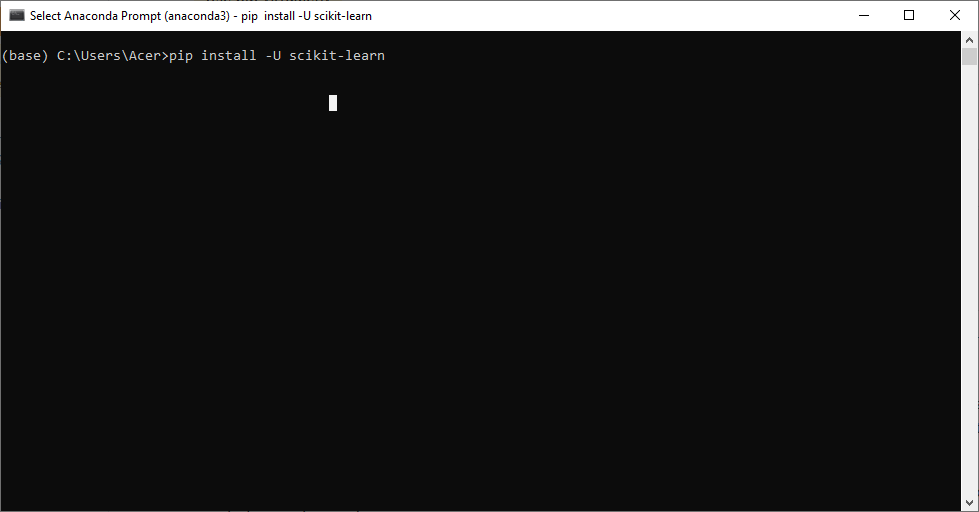
\includegraphics[scale=0.4]{figures/1.PNG}
		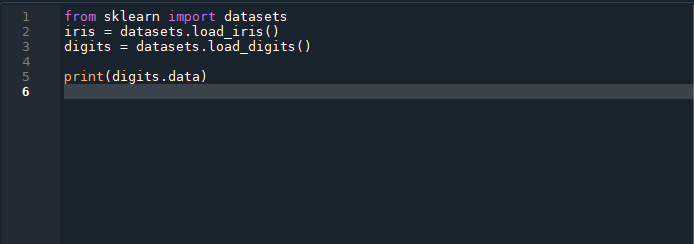
\includegraphics[scale=0.5]{figures/1a.PNG}
		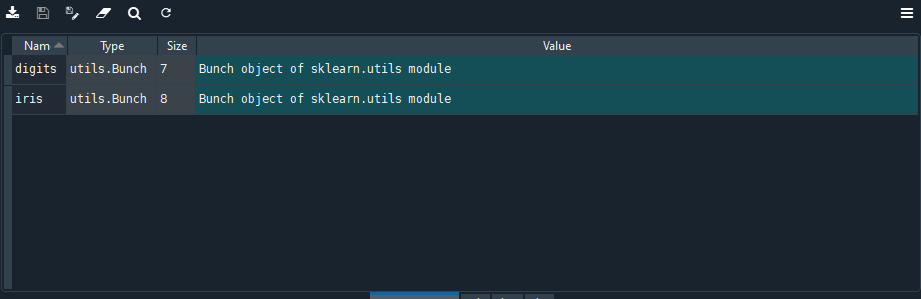
\includegraphics[scale=0.4]{figures/1b.PNG}
	\end{figure}

\newpage
\item
Mencoba Loading an example dataset, menjelaskan maksud dari tulisan tersebut dan mengartikan per baris.
	\begin{figure}[!htbp]
		\centering
		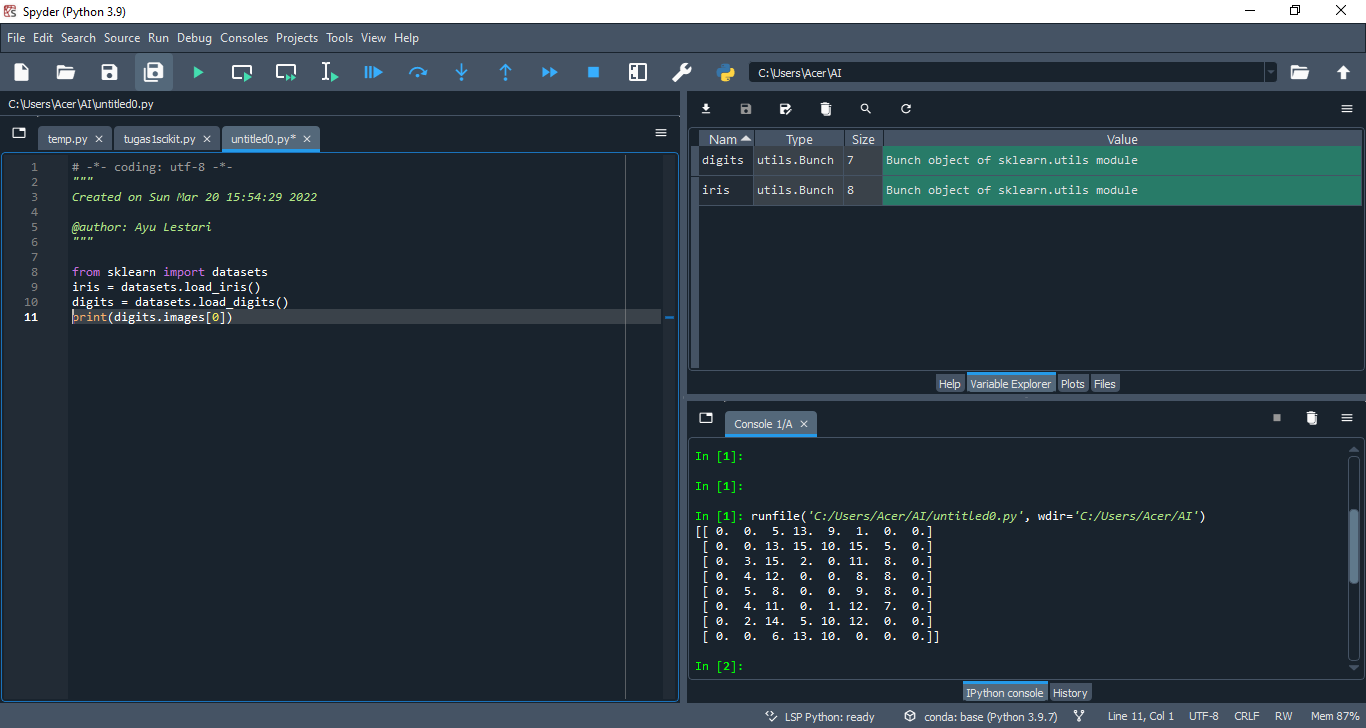
\includegraphics[scale=0.5]{figures/2.PNG}
		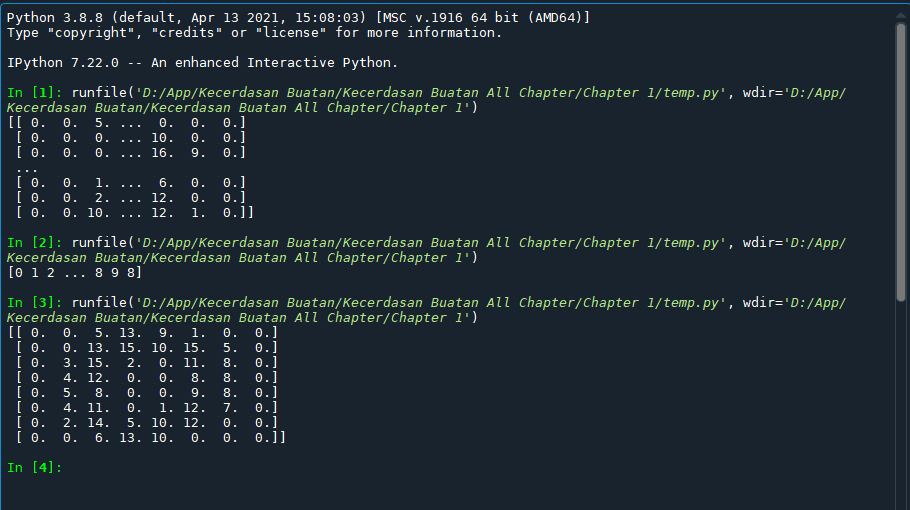
\includegraphics[scale=0.4]{figures/2a.PNG}
	\end{figure}

\newpage
\item
Mencoba Learning and predicting, menjelaskan maksud dari tulisan tersebut dan mengartikan per baris.
	\begin{figure}[!htbp]
		\centering
		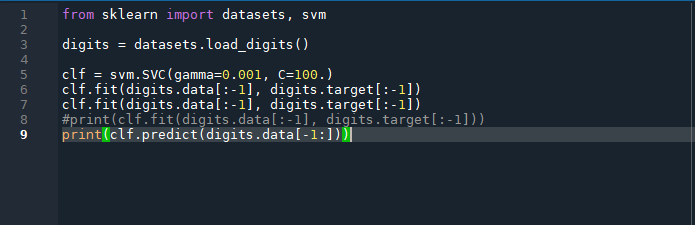
\includegraphics[scale=0.5]{figures/3.PNG}
		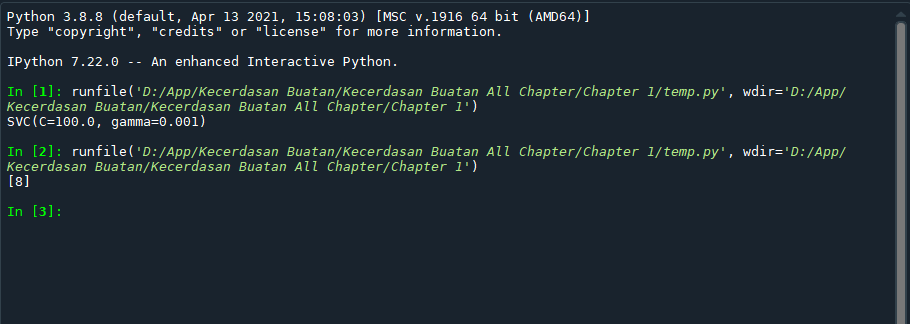
\includegraphics[scale=0.4]{figures/3a.PNG}
	\end{figure}


\item
Mencoba Model persistence, menjelaskan maksud dari tulisan tersebut dan mengartikan per baris. Terdapat dua cara yaitu menggunakan pickle atau menggunakan joblib.
	\begin{figure}[!htbp]
		\centering
		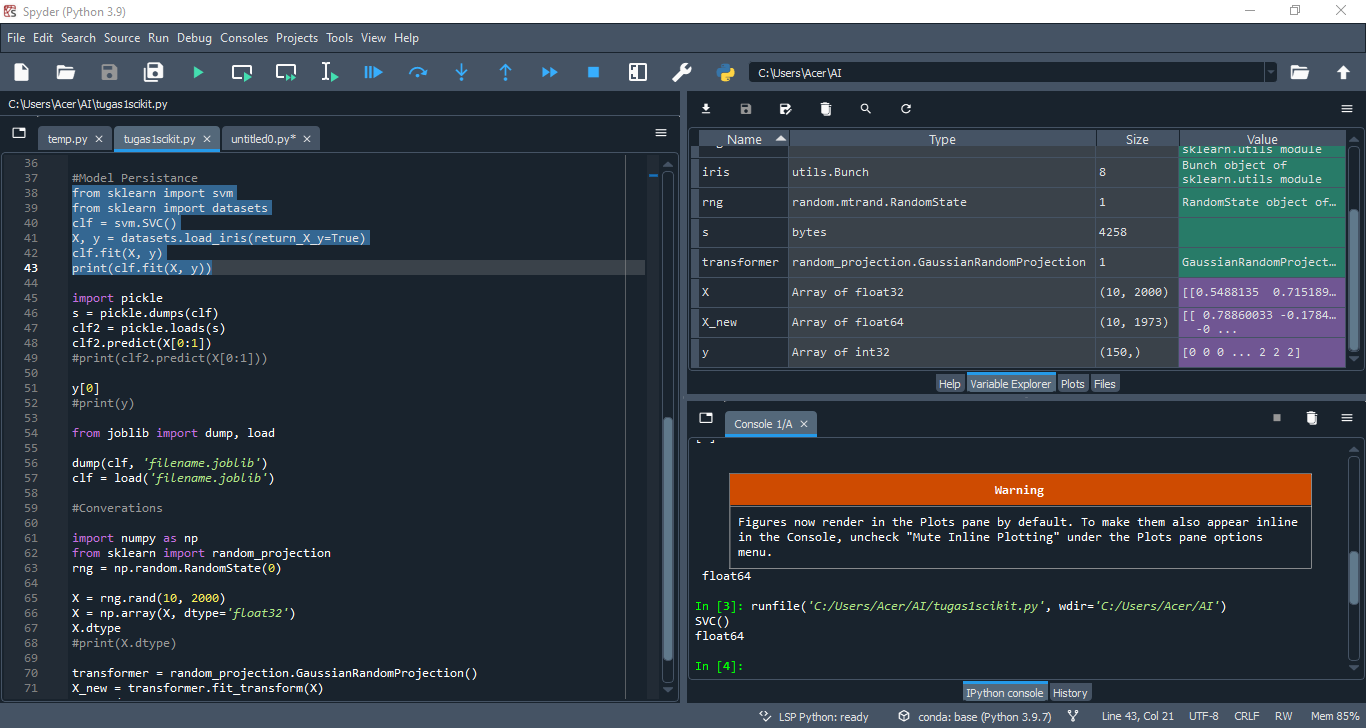
\includegraphics[scale=0.5]{figures/4.PNG}
		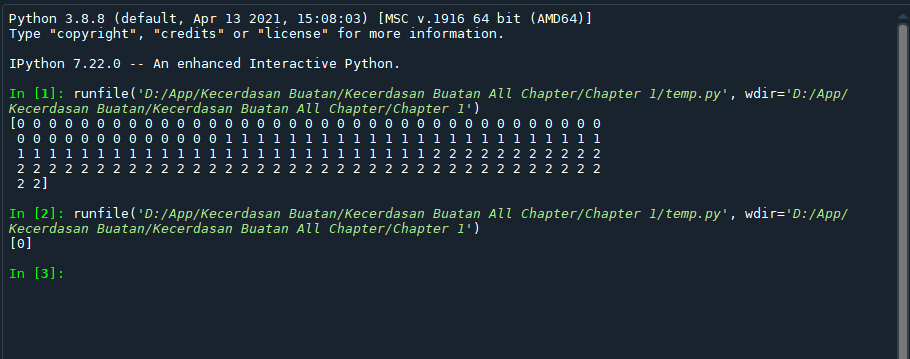
\includegraphics[scale=0.4]{figures/4a.PNG}
	\end{figure}

\newpage
\item 
Mencoba Conventions, menjelaskan maksud dari tulisan tersebut dan mengartikan per baris.
	\begin{figure}[!htbp]
		\centering
		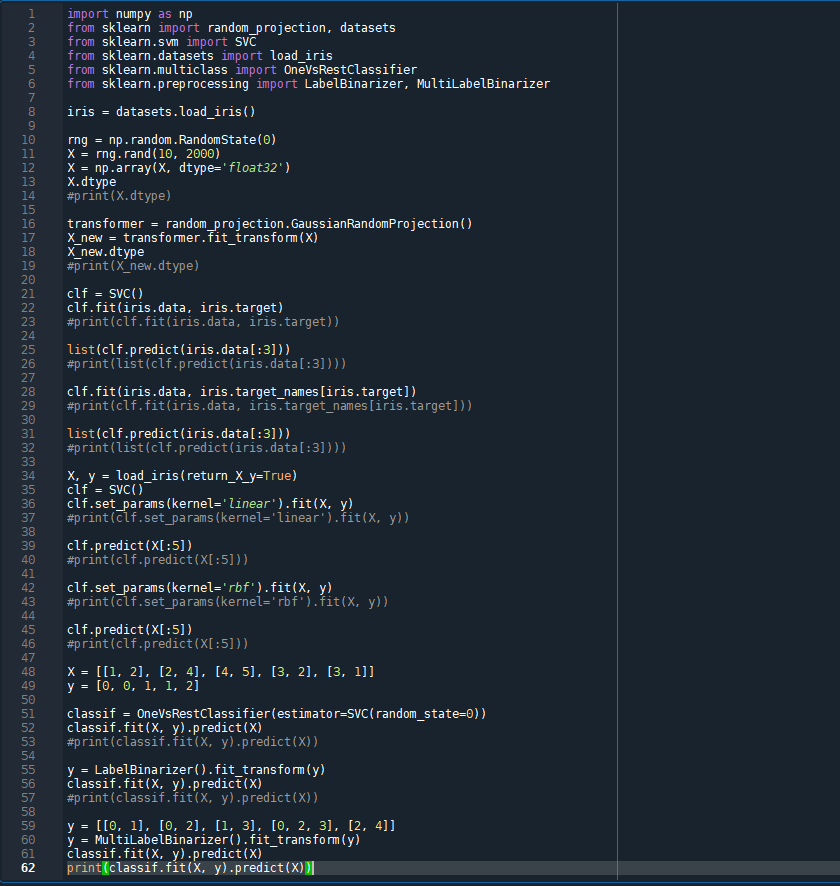
\includegraphics[scale=0.4]{figures/5.PNG}
		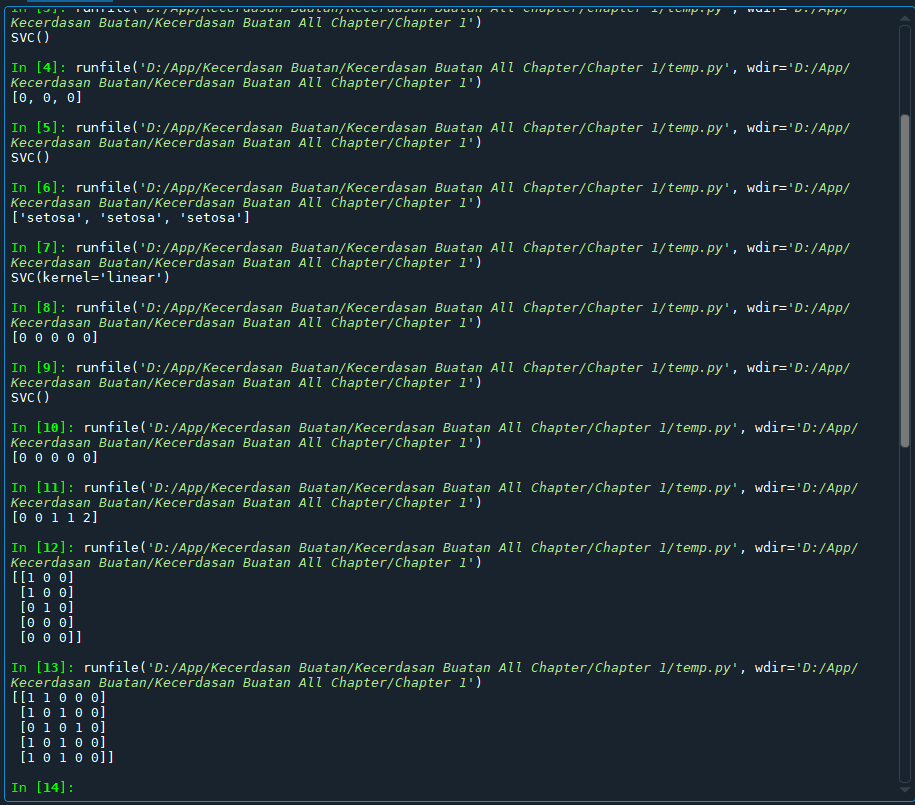
\includegraphics[scale=0.4]{figures/5a.PNG}
	\end{figure}

\end{enumerate}

\newpage
\section{Penanganan Error}
Dari percobaan yang dilakukan di atas, apabila mendapatkan error maka:

\begin{enumerate}
	\item Screenshot error.
	\begin{figure}[!htbp]
		\centering
		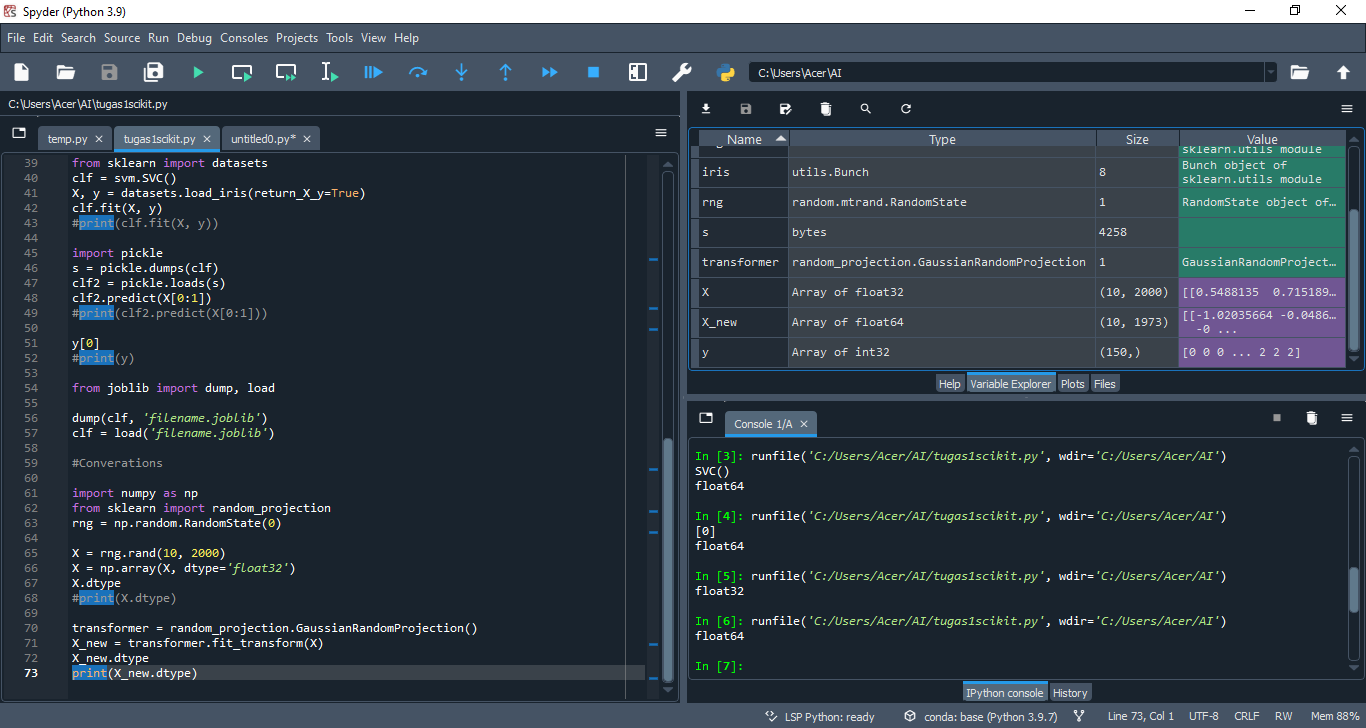
\includegraphics[scale=0.5]{figures/6.PNG}
		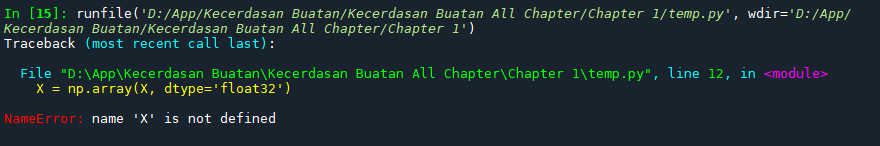
\includegraphics[scale=0.5]{figures/7.PNG}
	\end{figure}
	
	\item Tuliskan kode eror dan jenis errornya.
	\begin{enumerate}
		\item NotFittedError = This SVC instance is not fitted yet. Call ’fit’ with appropriate arguments before using this estimator.
		\item NameError = name ’X’ is not defined
	\end{enumerate}

	\item Solusi pemecahan masalah error tersebut.
	\begin{enumerate}
		\item NotFittedError = Solusinya yaitu memanggil parameter dengan method fit,
		sebelum menggunakan method predict.
		\item NameError = Solusinya yaitu membuat variabel dengan nama X.
	\end{enumerate}

\end{enumerate}

